\documentclass{article}

\usepackage{hyperref}
\usepackage[T1]{fontenc}
\usepackage{graphicx}
\usepackage{float}
\usepackage[utf8]{inputenc}


\title{%
Laboratorium 7\\
  \huge Kwadratury adaptacyjne}
\author{Mateusz Król}
\date{01/05/2024 r.}

\begin{document}
\maketitle

 
\section*{Zadanie 1.}
\textbf{Oblicz wartość całki z poprzedniego laboratorium
$$ \int_{0}^{1} \frac{4}{1+x^2} \,dx = \pi.$$
korzystając z:\\
(a) kwadratur adaptacyjnych trapezów,\\
(b) kwadratur adaptacyjnych Gaussa-Kronroda.\\\\
Dla każdej metody narysuj wykres wartości bezwzględnej błędu względnego w
zależności od liczby ewaluacji funkcji podcałkowej. Wyniki dodaj do wykresu
uzyskanego w poprzednim laboratorium.}
\newpage
Wykres funkcji $f(x) = \frac{4}{1+x^2}$:
\begin{figure}[H]
  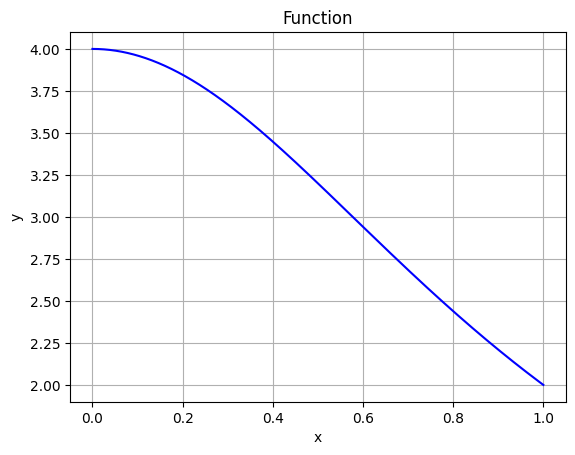
\includegraphics[width=\linewidth]{figures/f.png}
\end{figure}
Wykres błędów względnych w zależności od liczby ewaluacji
funkcji podcałkowej:
\begin{figure}[H]
  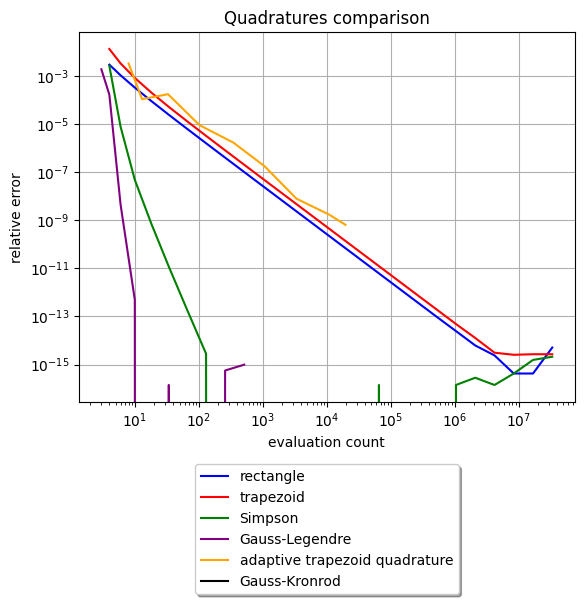
\includegraphics[width=\linewidth]{figures/quad_f.png}
\end{figure}
Wykres błędów względnych dla kwadratury \textit{Gaussa-Kronroda}
jest stale równy 0.
\\\\
\null\quad

\section*{Zadanie 2.}
\textbf{Powtórz obliczenia z poprzedniego oraz dzisiejszego laboratorium
dla całek:
$$ \int_{0}^{1} \sqrt[]{x}\cdot \ln(x) \,dx $$
$$ \int_{0}^{1} \frac{1}{(x-0.3)^2 + a} + \frac{1}{(x-0.9)^2 + b} - 6\,dx $$
, gdzie $a=0.001$, $b=0.004$.}
\newpage
Wykres funkcji $f(x) = \sqrt[]{x}\cdot \ln(x)$:
\begin{figure}[H]
  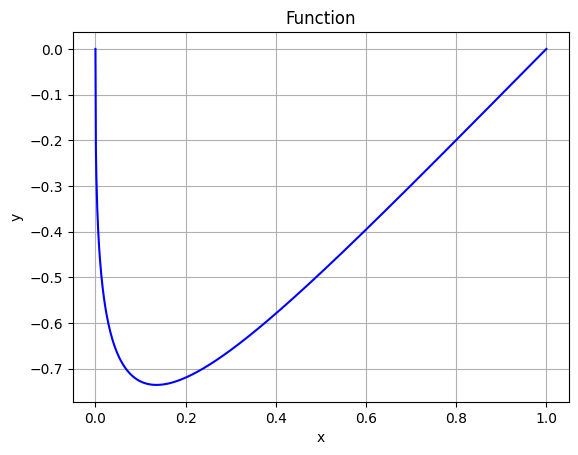
\includegraphics[width=\linewidth]{figures/g.png}
\end{figure}
Wykres błędów względnych w zależności od liczby ewaluacji
funkcji podcałkowej dla funkcji $f(x) = \sqrt[]{x}\cdot \ln(x)$:
\begin{figure}[H]
  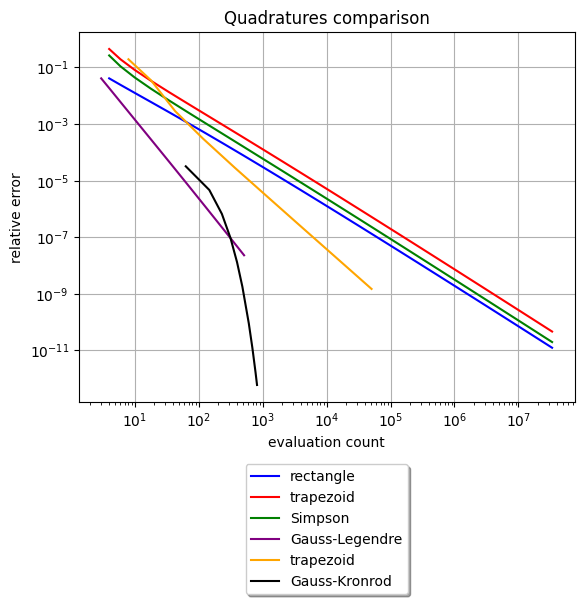
\includegraphics[width=\linewidth]{figures/quad_g.png}
\end{figure}

Wykres funkcji $f(x) = \frac{1}{(x-0.3)^2 + 0.001} + \frac{1}{(x-0.9)^2 + 0.004} - 6$:
\begin{figure}[H]
  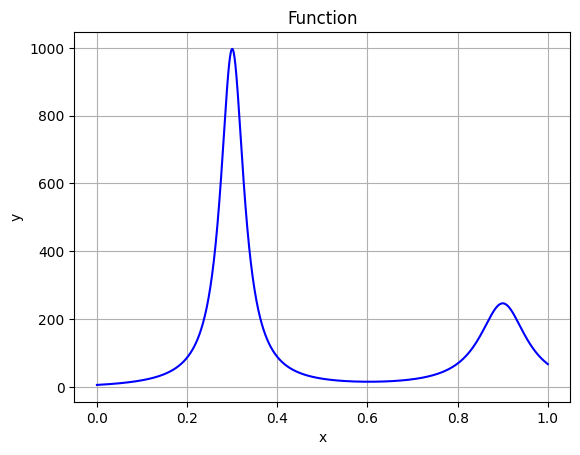
\includegraphics[width=\linewidth]{figures/h.png}
\end{figure}

Wykres błędów względnych w zależności od liczby ewaluacji
funkcji podcałkowej dla funkcji \space
$f(x) = \frac{1}{(x-0.3)^2 + 0.001} + \frac{1}{(x-0.9)^2 + 0.004} - 6$:
\begin{figure}[H]
  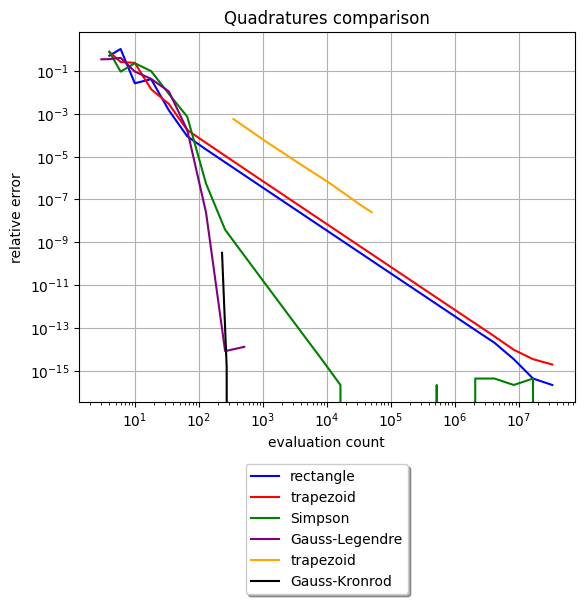
\includegraphics[width=\linewidth]{figures/quad_h.png}
\end{figure}


\subsection*{Wnioski}
\null\quad Dla każdej z badanej funkcji, metoda \textit{Gaussa-Kronroda} od
pewnej wartości liczby ewaluacji funkcji, przyjmuje najmniejszą wartość
względnego spośród wszystkich metod. \\
\null\quad W pierwszym zadaniu wartość błędu dla funkcji
$f(x)=\frac{4}{1+x^2}$ wyniósł 0, korzystając z wartości $\pi = numpy.pi$.\\
Oznacza to, że dokładność metody dla odpowiednich wartości
liczby ewaluacji funkcji (w tym przypadku stale równym 63), 
wynosi więcej niż 15 miejsc po przecinku. \\
\null\quad Dla drugiej badanej funkcji $f(x) = \sqrt[]{x}\cdot \ln(x)$,
wartości błędu względnego okazały się największe dla odpowiednich liczb ewaluacji
funkcji podcałkowej.

\end{document}